\documentclass{article}
\usepackage{fontspec}
\pagestyle{empty}
\usepackage{geometry}
\geometry{paperwidth=100mm, paperheight=100mm, left=2mm, top=0mm, right=2mm, bottom=0mm}
\parindent=0pt
\usepackage{color}
\usepackage{xcolor}
\usepackage{tikz}
\usetikzlibrary{positioning}

\begin{document}
\centering
\vspace*{\fill} \vspace*{-5ex}

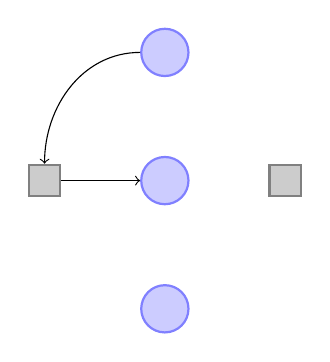
\begin{tikzpicture}[place/.style={circle,draw=blue!50,fill=blue!20,thick,
inner sep=0pt,minimum size=6mm},
transition/.style={rectangle,draw=black!50,fill=black!20,thick,
inner sep=0pt,minimum size=4mm}]
\node[place] (waiting) {};
\node[place] (critical) [below=of waiting] {};
\node[place] (semaphore) [below=of critical] {};
\node[transition] (leave critical) [right=of critical] {};
\node[transition] (enter critical) [left=of critical] {};
\draw [->] (enter critical) to (critical);
\draw [->] (waiting) to [out=180,in=90] (enter critical);
\end{tikzpicture}
\vspace*{\fill} 
\end{document}